\documentclass[12pt,twoside,vi]{mitthesis}
\usepackage{tikz}
\usepackage{circuitikz}
\usepackage{amsmath}
\begin{document}
\chapter{Network Sensing Algorithm}

Given access to the set of nodes in an electrical network, the objective of a network sensing algorithm is to determine the set of branches and the elements that compose them.
In order to illustrate how a network sensing algorithm operates, it is necessary to begin with a simple example and then build in complexity.  

\section{Grounding Clause}

Blah Blah

\section{Two Node Network}
Take the example of a network with two nodes below:

\begin{figure}[h]
  \begin{center}
    \begin{circuitikz}[american]
		\draw (0,3)
		node[label={right:$A$}] {}
		to[R=$R_{AB}$] (0,0)
		node[label={right:$B$}] {};
		\fill (0,3) circle (1mm);
		\fill (0,0) circle (1mm);
		
		\draw (3,0)
		to[short]
		node[sground] {} (3,0);
		\draw (3,0)
		to[V,v=$V_t$,i=$I_t$] (3,3)
		to[short](5,3)
		node[label={right:$A$}] {}
		to[R=${R_{AB}=\frac{V_t}{I_t}}$] (5,0)
		node[label={right:$B$}] {}
		to[short](3,0); 
		
		\draw (9,0)
		to[short]
		node[sground] {} (9,0);
		\draw (9,0)
		to[V,v=$V_t$,i=$I_t$] (9,3)
		to[short](11,3)
		node[label={right:$B$}] {}
		to[R=${R_{BA}=\frac{V_t}{I_t}}$] (11,0)
		node[label={right:$A$}] {}
		to[short](9,0);
		\fill (5,3) circle (1mm);
		\fill (5,0) circle (1mm);
		\fill (11,3) circle (1mm);
		\fill (11,0) circle (1mm);
    \end{circuitikz}
   \caption{Finding $R_{AB}$ in a two node network}
  \end{center}
\end{figure}

In the case of a resistive network with two nodes, there is only one possible branch in the network and thus one possible element to characterize.
From elementary circuit theory, the resistance between two nodes equal to the voltage across the nodes divided by the current through the nodes when power is applied.  
Here, the resistance $R_{AB}$ is found by placing a test voltage $V_t$ across the nodes and measuring the resulting current, $I_t$, then taking the ratio $\frac{V_t}{I_t}$.
This measurement is called the driving point impedance \footnote{To measure a driving point impedance, a test voltage is applied between the node of interest and ground, and the resulting current in the voltage source is measured. 
The driving point impedance is then computed by dividing the test voltage by the resulting current.}.
If there are no circuit elements between the two nodes, the driving point impedance test will find zero current in the test voltage source, resulting in an infinite resistance between two nodes.
An infinite resistance between two nodes in a circuit indicates that there are no elements in that branch of the network.
Thus, the network can subsequently be simplified by removing that branch from the network.


\section{Three Node Network}

A resistive network with two nodes is simple, but provides an introduction to the methodology used in analyzing larger networks.
In the case of a resistive network with three nodes, it is insufficient to utilize driving point impedance measurements alone, because each node has more than one path to any other node.
%Taking the driving point impedance at any node returns a parallel combination of the set of branch resistors, depending on which nodes are grounded.
\begin{figure}[h]
  \begin{center}
    \begin{circuitikz}[american]
    	\ctikzset{label/align = straight}
    	\def\offset{0}
		\draw (\offset,0)
		node[label={above:$A$}] {}
		to[R, l=$R_{AB}$] (3+\offset,0)
		node[label={above:$B$}] {}
		to[R, l=$R_{BC}$] (1.5+\offset,-2.548)
		node[label={right:$C$}] {}
		to[R, l=$R_{AC}$] (0+\offset,0);
		\fill (\offset,0) circle (1mm);
		\fill (1.5+\offset,-2.584) circle (1mm);
		\fill (3+\offset,0) circle (1mm);
		
		\def\offset{5.5}
		\draw (-1+\offset,-2.548)
		to[short]
		node[sground] {} (-1+\offset,-2.548);
		\draw (-1+\offset,-2.548)
		to[V,v=$V_t$,i=$I_t$] (-1+\offset,0)
		to[short](0+\offset,0);
		\draw (\offset,0)
		node[label={above:$A$}] {}
		to[R, l=$R_{AB}$] (3+\offset,0)
		node[label={above:$B$}] {}
		to[R, l=$R_{BC}$] (1.5+\offset,-2.548)
		node[label={right:$C$}] {}
		to[R, l=$R_{AC}$] (0+\offset,0);
		\draw (1.5+\offset,-2.548)
		to[short]
		node[sground] {} (1.5+\offset,-2.548);
		\draw (3+\offset,0)
		to[short] (4+\offset,0)
		to[short] (4+\offset,-2.548)
		node[sground] {};
		\fill (\offset,0) circle (1mm);
		\fill (1.5+\offset,-2.584) circle (1mm);
		\fill (3+\offset,0) circle (1mm);
		
		\def\offset{12}
		\draw (-1+\offset,-2)
		to[short,o-] (-1+\offset,-2.548)
		node[sground] {} (-1+\offset,-2.548);
		\draw (-.75+\offset,-2)
		to[open,v^>=$V_A$] (-.75+\offset,-.1)
		to[open](-1+\offset,0)
		to[short,o-](0+\offset,0);
		\draw (\offset,0)
		node[label={above:$A$}] {}
		to[R, l=$R_{AB}$] (3+\offset,0)
		node[label={above:$B$}] {}
		to[R, l=$R_{BC}$] (1.5+\offset,-2.548)
		node[label={right:$C$}] {}
		to[R, l=$R_{AC}$] (0+\offset,0);
		\draw (1.5+\offset,-2.548)
		to[short]
		node[sground] {} (1.5+\offset,-2.548);
		\draw (4+\offset,-2.548)
		node[sground] {}
		to[V,v_>=$V_t$] (4+\offset,0)
		to[short] (3+\offset,0)
		;
		\fill (\offset,0) circle (1mm);
		\fill (1.5+\offset,-2.584) circle (1mm);
		\fill (3+\offset,0) circle (1mm);
		
    \end{circuitikz}
   \caption{Finding $R_{AB}$ in a three node network}
  \end{center}
\end{figure}

Consider a resistive network with three nodes: A, B, and C. 
In order to determine the resistance in branch AB, the driving point impedance at node A is measured with nodes B and C grounded. 
This provides the resistance of the parallel combination of the branches with an endpoint at node A,\\
$R_{A_{||}} = R_{AB}||R_{AC}$.
\footnote
{$
	\displaystyle R_{1}||R_{2} = 
	\frac{R_{1}R_{2}}{R_{1}+R_{2}}
$}
Next, a test voltage source is applied to node B, node C is grounded, and the voltage at node A, $V_A$, is observed.
$\displaystyle V_{A} = V_t
\frac{R_{AC}} {R_{AB}+R_{AC}} = V_t
\frac{R_{AB}||R_{AC}} {R_{AB}} = V_t
\frac{R_{A_{||}}} {R_{AB}}
$\\
The branch resistance of interest, $R_{AB}$ is calculated using the known quantities $V_t$, $V_{A{||}}$, and $V_A$.
$\displaystyle R_{AB} = 
V_t\frac{R_{A{||}}} {V_A}$ \\
This procedure is repeated for the remaining branches to determine the entire network.


\section{N Node Network}

A resistive network with any number of nodes can be reduced to a resistive network with three nodes by grounding the nodes that are not of interest.
The resulting network does not modify the branch of interest, but connects the remaining branches attached to the nodes of interest in parallel.
This collapses the network into a three node network or three branch equivalent circuit.
\begin{figure}[h]
  \begin{center}
    \begin{circuitikz}
    %\ctikzset{label/align = straight}
		\draw (0,0)
		node[label={above:$A$}] {}
		to[R, l=$R_{AC}$] (1.5,-2.584)
		node[label={below:$C$}] {}
		to[R, l=$R_{EC}$] (3,0) % The resistor
		node[label={above:$E$}] {}
		to[R, l_=$R_{AE}$] (0,0)
		to[R, l^=$R_{AB}$] (-1.5,-2.584)
		node[label={below:$B$}] {}
		to[R, l_=$R_{BC}$] (1.5,-2.584)
		to[R, l_=$R_{CD}$] (4.5,-2.584)
		node[label={below:$D$}] {}
		to[R, l=$R_{ED}$] (3,0);
		\fill (0,0) circle (1mm);
		\fill (3,0) circle (1mm);
		\fill (1.5,-2.584) circle (1mm);
		\fill (4.5,-2.584) circle (1mm);
		\fill (-1.5,-2.584) circle (1mm);
    \end{circuitikz}
   \caption{Five node network}
  \end{center}
\end{figure}
Consider a resistive network with five nodes: A-E.  
To determine the resistance between nodes A and E, the network is reduced to a three-node network by connecting all nodes except nodes A and E to ground.
The three resistances of the branches that remain are $R_{AE}$, $R_{AB}||R_{AC}$, and $R_{EC}||R_{ED}$.
The reduced network is then solved using the three node network method, and this procedure is repeated for all branches in the network.

\section{Element Identification}

Networks composed of elements with complex impedance can be analyzed with the same algorithm.
By replacing the test DC voltage sources with AC voltage sources, the imaginary reactance of capacitors and inductors can be measured in addition to the real resistance of resistors.

\subsection{From Resistance to Impedance}

Chapter 2 described the use of the Laplace Transform to characterize the behavior of circuit elements in the frequency domain.
Here, frequency-domain complex impedance is useful for identifying circuit elements based on the change in branch impedance over inputs of various frequencies.


MAKE NOTE ABOUT USING THE AMPLITUDE OF THE MEASURED SIGNALS

\subsection{Parallel RLC Branches}

To determine if there are multiple element types [in parallel] between two nodes, we can select a few frequencies to scan through and analyze the resulting change in impedance.

\begin{figure}[h]
  \begin{center}
    \begin{circuitikz}
		\draw (0,-.5)
		node[label={below:$2$}] {}
		to[short] (0,0)
		to[R=$R$] (0,2)
		to[short] (1.5,2)
		to[L=$L$] (1.5,0) % The resistor
		to[short] (-1.5,0)
		to[C=$C$] (-1.5,2)
		to[short] (0,2)
		to[short] (0,2.5)
		node[label={above:$1$}] {};
	    \fill (0,-.5) circle (1mm);
		\fill (0,2.5) circle (1mm);
    \end{circuitikz}
   \caption{Example RLC Tank Circuit}
  \end{center}
\end{figure}

The impedance of a parallel RLC 'tank' circuit can be characterized and analyzed over all frequencies.

\begin{align}
Z_C = \frac{1}{j\omega C} \qquad Z_R = R \qquad Z_L = j\omega L \\
Z_{RLC}=Z_C||Z_R||Z_L = \frac{1}{j\omega C+\frac{1}{R}+\frac{1}{j\omega L}}= \frac{j\omega RL}{-\omega^2RLC+j\omega L+R}
\end{align}

$\displaystyle Z_{RLC}$ has a zero at $\frac{1}{RL}$ and two poles at $\frac{-L^{+}_{-}\sqrt{L^2+4R^2LC}}{-2RLC}$\\
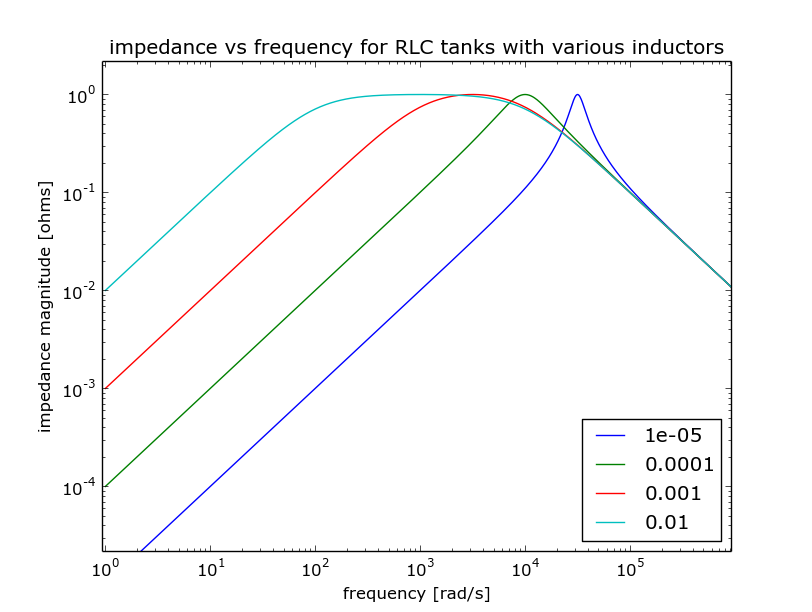
\includegraphics[width=0.35\textwidth]{../inductors.png}
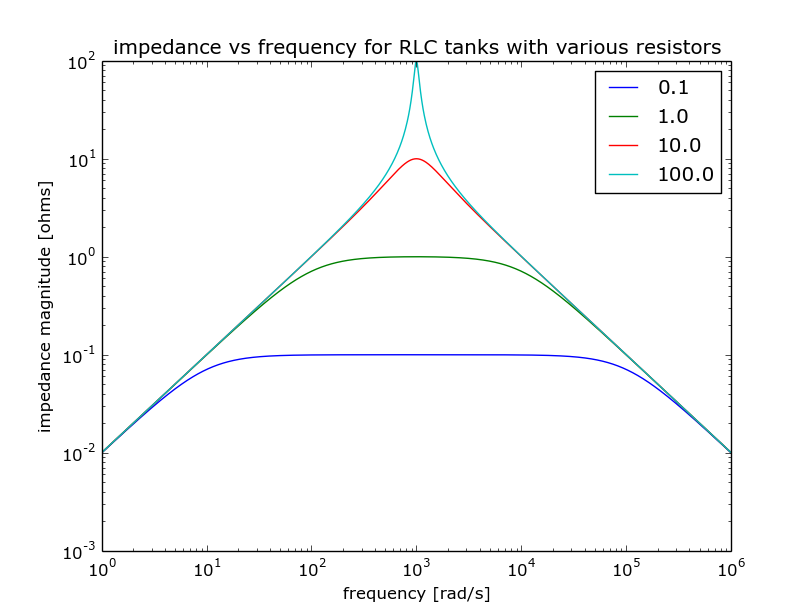
\includegraphics[width=0.35\textwidth]{../resistors.png}
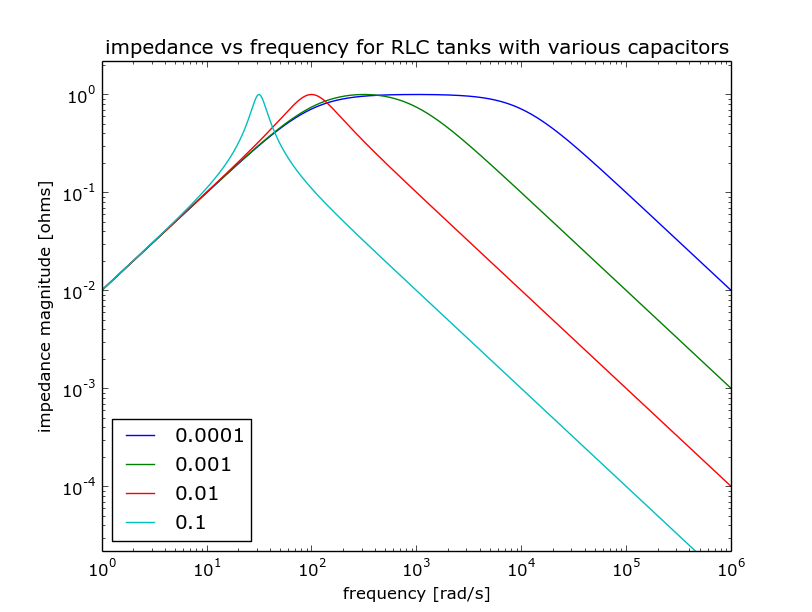
\includegraphics[width=0.35\textwidth]{../capacitors.png}\\
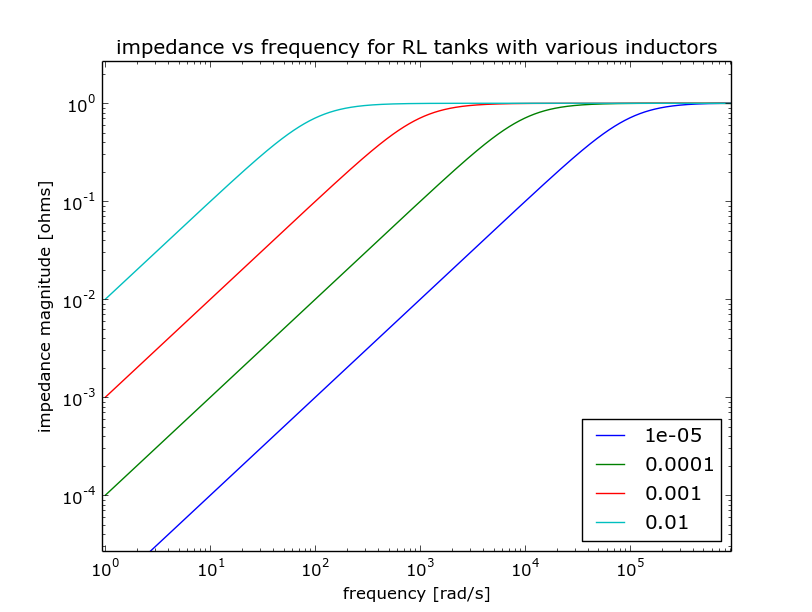
\includegraphics[width=0.35\textwidth]{../rL.png}
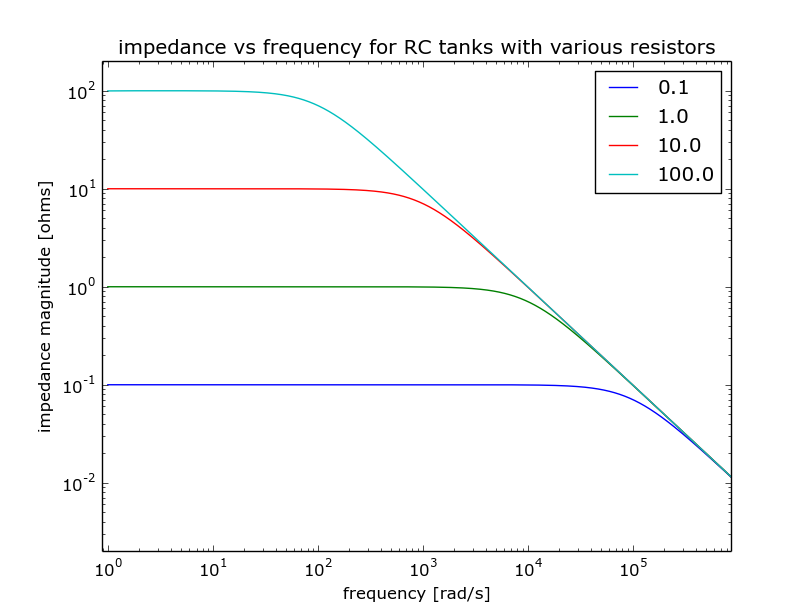
\includegraphics[width=0.35\textwidth]{../Rc.png}
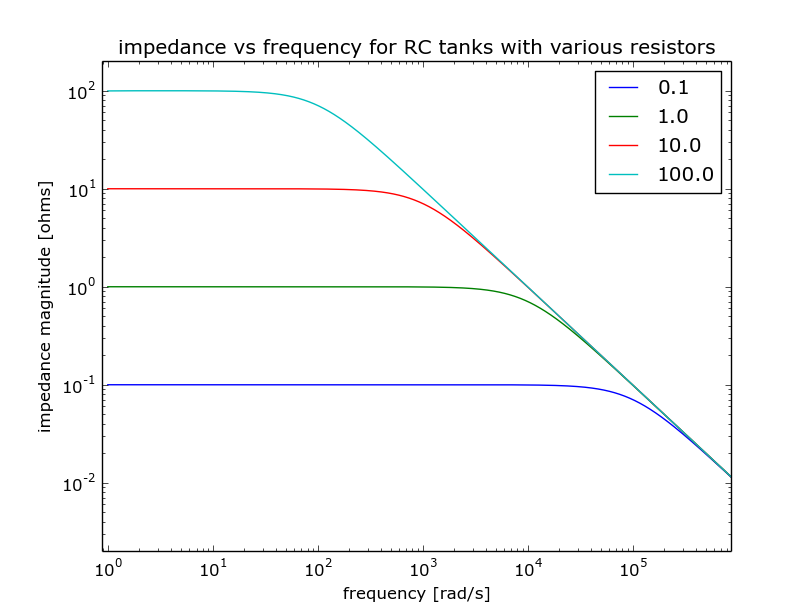
\includegraphics[width=0.35\textwidth]{../rC.png}\\


If we look at the plots above, we can see that varying the resistance changes the maximum impedance over all frequencies, varying the inductance drops the asymptotic impedance at low frequencies, and varying the capacitance drops the asymptotic impedance at high frequencies.
We can imagine there are three regimes on the impedance vs frequency plot that divide the operation of an RLC tank into three elements:\\
When the slope is +1, the tank behaves like an inductor
$L=|Z|/(j\omega)$.
When the slope is -1, the tank behaves like a capacitor
$C=j\omega |Z|$.
When the slope is 0, the tank behaves like a resistor
$R=|Z|$.


\subsection{Finite Difference Stencil}
To reliably determine the regions of effective resistance, inductance, and capacitance, the slope of the $log{|Z_{nm}|}$ vs. $log{(\omega)}$ is computed via the Midpoint Method.
The Midpoint Finite Difference Stencil takes the two points on either side of the point of interest and computes the slope between them.
Z'[n]=$\frac{1}{2}$(Z[n+1]-Z[n-1]).

\subsection{Component Value Calculation}
Once the regions of the impedance plot are identified and assigned to component, the component value is calculated for each sample taken on the impedance plot:\\
$R = Z[\omega]\\
L = \frac{Z[\omega]}{\omega}\\
C = \frac{1}{\omega Z[\omega]} 
$ 

The resulting resistances, inductances, and capacitances are averaged to counter noisy data.


\section{Reconstructing the Network}
With a record of all of the elements and their connections in the network, the network is reconstructed.
\end{document}